% ============================================================
% HSBI Beamer — ISLP Lecture Series — IMPROVED EDITION
% Chapter 8: Tree-Based Methods
% ============================================================
\documentclass[aspectratio=169,11pt]{beamer}
\usepackage[utf8]{inputenc}\usepackage[T1]{fontenc}\usepackage[english]{babel}
\usepackage{graphicx}\usepackage{booktabs}\usepackage{amsmath,amssymb,amsfonts}
\usepackage{mathtools}\usepackage{hyperref}\usepackage{xcolor}
\usepackage{verbatim}\usepackage{alltt}
\usepackage{tikz}\usetikzlibrary{calc,arrows.meta,positioning,shapes}
\usepackage{tcolorbox}\tcbuselibrary{skins}

\usetheme{Madrid}\usecolortheme{default}
\setbeamertemplate{navigation symbols}{}
\setbeamertemplate{footline}[frame number]
\setbeamertemplate{blocks}[rounded][shadow=false]
\setbeamertemplate{headline}{%
  \leavevmode\hbox{%
    \begin{beamercolorbox}[wd=\paperwidth,ht=2.2ex,dp=0.9ex]{section in head/foot}%
      {\fontsize{4.6}{5.2}\selectfont%
       \insertsectionnavigationhorizontal{\paperwidth}{}{\hskip0pt plus1filll}}%
    \end{beamercolorbox}}%
}
\setbeamerfont{section in head/foot}{size=\tiny}
\setbeamerfont{palette primary}{size=\tiny}
\setbeamerfont{palette tertiary}{size=\tiny}
\setbeamerfont{section in toc}{size=\footnotesize}

\usepackage{listings}
\definecolor{pyKw}{RGB}{0,0,180}\definecolor{pyStr}{RGB}{20,120,40}
\definecolor{pyCom}{RGB}{120,120,120}\definecolor{accent}{RGB}{38,70,140}
\lstdefinestyle{Pystyle}{language=Python,basicstyle=\ttfamily\footnotesize,
  keywordstyle=\color{pyKw}\bfseries,commentstyle=\color{pyCom}\itshape,
  stringstyle=\color{pyStr},showstringspaces=false,upquote=true,
  columns=fullflexible,breaklines=true,literate={~}{{$\sim$}}1}
\lstset{style=Pystyle}

\AtBeginSection[]{\begin{frame}{Outline}\footnotesize
  \tableofcontents[currentsection,sectionstyle=show/shaded,subsectionstyle=show/show/hide]
\end{frame}}

\newcommand{\islpsource}[1]{%
  \vfill\hfill{\tiny\itshape\color{gray}Source: #1 \textemdash{} ISLP, James et al.\ (2023).}\par
}

\newtcolorbox{takeaway}[1][Takeaway]{enhanced,colback=green!4,colframe=green!50!black,
  boxrule=0pt,leftrule=2.5pt,arc=2pt,fonttitle=\bfseries,title=#1,
  left=2mm,right=2mm,top=1mm,bottom=1mm}
\newtcolorbox{numexample}[1][Worked example]{enhanced,colback=orange!4,colframe=orange!70!black,
  boxrule=0pt,leftrule=2.5pt,arc=2pt,fonttitle=\bfseries,title=#1,
  left=2mm,right=2mm,top=1mm,bottom=1mm}
\newtcolorbox{readme}[1][How to read this]{enhanced,colback=blue!4,colframe=accent,
  boxrule=0pt,leftrule=2.5pt,arc=2pt,fonttitle=\bfseries,title=#1,
  left=2mm,right=2mm,top=1mm,bottom=1mm}

\title{An Introduction to Statistical Learning}
\subtitle{Chapter 8: Tree-Based Methods \textemdash{} Improved Edition}
\author{Prof.\ Dr.\ Christoph Weisser}\institute{HSBI}
\date{Summer Semester 2026}\graphicspath{{images/}}

\newtcolorbox{exercise}[1][Exercise]{enhanced, fontupper=\footnotesize, colback=purple!4, colframe=purple!55!black, boxrule=0pt, leftrule=2.5pt, arc=2pt, fonttitle=\bfseries, title=#1, left=2mm, right=2mm, top=1mm, bottom=1mm}
\newtcolorbox{solutionbox}[1][Solution]{enhanced, fontupper=\footnotesize, colback=teal!5, colframe=teal!55!black, boxrule=0pt, leftrule=2.5pt, arc=2pt, fonttitle=\bfseries, title=#1, left=2mm, right=2mm, top=1mm, bottom=1mm}
\newtcolorbox{longexercise}[1][Extended exercise (15 min)]{enhanced, fontupper=\footnotesize, colback=violet!6, colframe=violet!55!black, boxrule=0pt, leftrule=3pt, arc=2pt, fonttitle=\bfseries, title=#1, left=2mm, right=2mm, top=1mm, bottom=1mm}

% Reclaim ~2pt of body height (custom nav headline makes full slides tip over by ~1.83pt)
\addtobeamertemplate{frametitle}{}{\vspace{-2pt}}

\newtcolorbox{labnote}[1][Run this live in the lab notebook]{enhanced, fontupper=\footnotesize, colback=cyan!7, colframe=cyan!45!black, boxrule=0pt, leftrule=3pt, arc=2pt, fonttitle=\bfseries, title=#1, left=2mm, right=2mm, top=1mm, bottom=1mm}

\begin{document}
\begin{frame}[plain]\titlepage\end{frame}

\begin{frame}{The course at a glance}
  \footnotesize
  \begin{center}
  \begin{tabular}{@{}c r l@{}}
    & \textbf{Lecture} & \textbf{Topic}\\
    \midrule
     & 1 & Ch.\ 1 + 2 --- Introduction; what is statistical learning \\
     & 2 & Ch.\ 2 --- Accuracy, bias--variance, Bayes classifier, KNN \\
     & 3--4 & Ch.\ 3 --- Linear regression (estimation, inference, diagnostics) \\
     & 5--6 & Ch.\ 4 --- Classification (logistic, LDA/QDA, naive Bayes, ROC) \\
     & 7 & Ch.\ 5 --- Resampling (validation, CV, bootstrap) \\
     & 8 & Ch.\ 6 --- Model selection and regularisation (ridge, lasso) \\
     & 9 & Ch.\ 7 --- Moving beyond linearity (splines, GAMs) \\
    $\blacktriangleright$ & \textbf{10} & \textbf{Ch.\ 8 --- Tree-based methods (trees, forests, boosting)} \\
     & 11 & Ch.\ 10 --- Deep learning (MLPs, CNNs, training) \\
     & 12 & Ch.\ 13 --- Multiple testing (FWER, FDR) \\
  \end{tabular}
  \end{center}
  \vspace{2pt}
  {\scriptsize Twelve sessions of 180 minutes. $\blacktriangleright$ marks today's chapter. Short exercises every $\sim$20 min; extended exercises every $\sim$45 min; each chapter has a companion lab notebook.}
\end{frame}


\begin{frame}{Contents}\small
  \tableofcontents[hideallsubsections]
\end{frame}

\begin{frame}{Notation in this chapter}
  \footnotesize
  \begin{center}
  \begin{tabular}{@{}ll@{}}
    \toprule
    \textbf{Symbol} & \textbf{Meaning} \\
    \midrule
    $R_j$ & Rectangular region (leaf) of the partitioned predictor space \\
    $\bar y_{R_j}$ & Mean training response in region $R_j$ (leaf prediction) \\
    $J$, $|T|$ & Number of leaves of a tree $T$ (its complexity) \\
    $\alpha$ & Cost-complexity pruning parameter: price paid per leaf \\
    $\hat p_{mk}$ & Fraction of node-$m$ training points in class $k$ \\
    $G$ & Gini index $\sum_k \hat p_{mk}(1-\hat p_{mk})$: node impurity \\
    $D$ & Cross-entropy $-\sum_k \hat p_{mk}\log\hat p_{mk}$: node impurity \\
    $B$ & Number of bootstrap samples / trees in an ensemble \\
    $m$ & Predictors tried per split in a random forest ($m=p$: bagging) \\
    $\rho$ & Pairwise correlation between the ensemble's trees \\
    $\lambda$ (or $\nu$), $d$ & Boosting learning rate (shrinkage) and tree depth \\
    \bottomrule
  \end{tabular}
  \end{center}
\end{frame}

\begin{frame}{Sources and references}
  \begin{block}{Primary textbook}
    James et al.\ (2023). \emph{An Introduction to Statistical Learning,
    with Applications in Python.} Springer.
  \end{block}
  \begin{block}{About this improved edition}
    Each method is introduced with motivation, intuition, formal
    definition, and worked examples. Slide titles are descriptive.
  \end{block}
\end{frame}

\begin{frame}{Learning objectives for this chapter}
  By the end of this chapter you will be able to:
  \begin{itemize}
    \item \textbf{Build} regression and classification trees by
          recursive binary splitting; \textbf{apply} cost-complexity
          pruning.
    \item \textbf{Explain} why a single tree is high-variance and how
          \emph{bagging} reduces that variance.
    \item \textbf{Distinguish} bagging from random forests; explain
          the benefit of feature subsampling at each split.
    \item \textbf{State} the boosting algorithm and its three tuning
          parameters.
    \item \textbf{Choose} between trees, random forests, and boosting
          for a given tabular problem.
  \end{itemize}
\end{frame}


\begin{frame}{Roadmap of this chapter}
  \begin{takeaway}[From single trees to industrial ensembles]
    \begin{enumerate}
      \item Single trees: regression and classification, pruning.
      \item Bagging: variance reduction by averaging.
      \item Random forests: bagging plus feature subsampling.
      \item Boosting: sequential additive trees on residuals.
      \item BART: Bayesian sum of trees.
    \end{enumerate}
  \end{takeaway}
\end{frame}

% ============================================================
\section{Why this chapter matters}
% ============================================================

\begin{frame}{Why trees dominate tabular data}
  Tree-based methods are the dominant non-linear method on tabular
  data.
  \begin{takeaway}[Five reasons]
    \begin{itemize}
      \item Capture nonlinearity \emph{and} interactions automatically.
      \item Interpretable as a sequence of yes/no questions.
      \item Handle mixed predictor types without dummy coding.
      \item Robust to outliers and monotone transformations.
      \item Ensembles (random forests, gradient boosting) routinely
            win Kaggle competitions on tabular data.
    \end{itemize}
  \end{takeaway}
\end{frame}

\begin{frame}{Single trees are weak: ensembles fix it}
  \begin{alertblock}{The single-tree pathology}
    A single tree is high-variance, blocky, and unstable. Small data
    changes produce very different trees.
  \end{alertblock}
  \begin{takeaway}
    The fix is to build many trees and aggregate. Bagging, random
    forests, gradient boosting, and BART all do this --- in different
    ways.
  \end{takeaway}
\end{frame}


% ============================================================
\section{Trees}
% ============================================================

\begin{frame}{Regression trees: idea}
  A regression tree is a piecewise-constant predictor over a partition
  of the predictor space.
  \begin{block}{The two-step view}
    \begin{enumerate}
      \item Partition the predictor space into $J$ rectangular regions
            $R_1, \ldots, R_J$.
      \item Predict the mean response $\bar y_{R_j}$ on each region.
    \end{enumerate}
  \end{block}
  \begin{block}{Goal}
    Minimise within-region variability:
    $\sum_{j = 1}^J \sum_{i \in R_j} (y_i - \bar y_{R_j})^2$.
  \end{block}
\end{frame}

\begin{frame}{Reading the tree-fit objective}
  \begin{readme}
    \begin{tabular}{@{}cl@{}}
      \toprule
      \textbf{Symbol} & \textbf{Meaning} \\
      \midrule
      $J$ & Number of leaves (regions) \\
      $R_j$ & Rectangular region in $\mathbb{R}^p$ \\
      $\bar y_{R_j}$ & Mean of $y$-values inside region $j$ \\
      \bottomrule
    \end{tabular}
  \end{readme}
  \begin{takeaway}
    Finding the globally optimal partition is computationally
    infeasible. In practice we use \emph{recursive binary splitting}.
  \end{takeaway}
\end{frame}

\begin{frame}{Recursive binary splitting: one step}
  \begin{block}{The greedy step}
    At each node:
    \begin{enumerate}
      \item For every predictor $X_j$ and every cutpoint $s$, compute
            the RSS that would result from splitting on $X_j < s$.
      \item Pick the $(j, s)$ that minimises the resulting RSS.
      \item Recurse on each child.
    \end{enumerate}
  \end{block}
  \begin{readme}[Greedy growth and stopping rules]
    ``Greedy'' means each split optimises the \emph{current} node only,
    never looking ahead --- fast, but not the globally optimal tree
    (hence grow-then-prune). Stop on minimum leaf size, maximum depth,
    or minimum RSS gain.
  \end{readme}
\end{frame}

\begin{frame}{Hitters: a baseball-salary tree}
  \begin{center}
    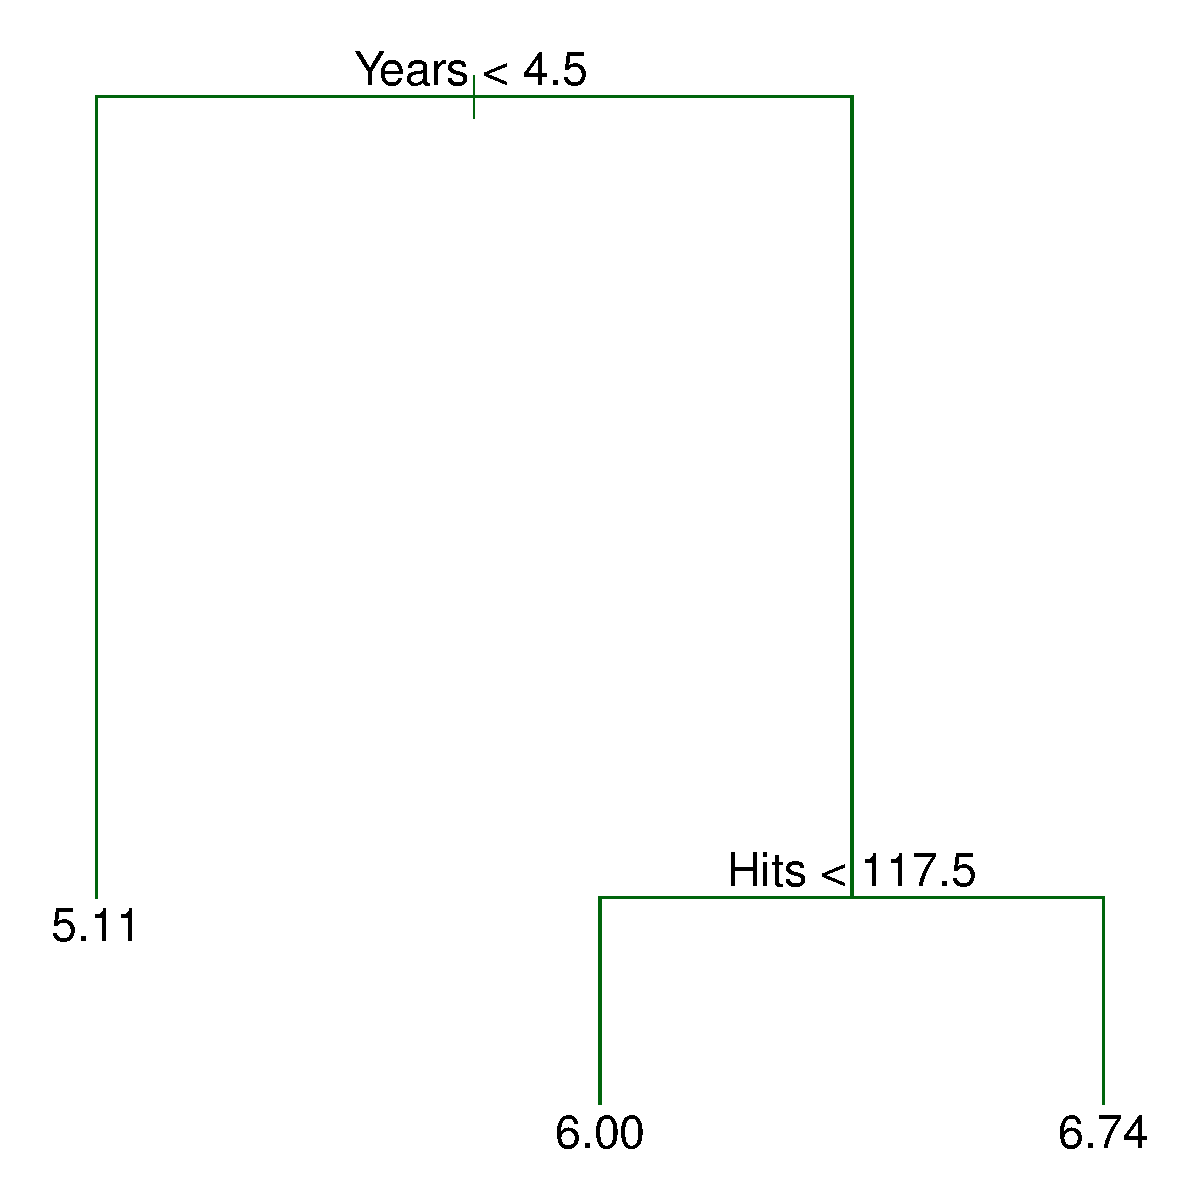
\includegraphics[width=0.85\textwidth,height=0.66\textheight,keepaspectratio]{8_1.pdf}
  \end{center}
  Years and Hits split the salary space into three regions; each leaf
  predicts the regional mean log-salary.
  \islpsource{Figure 8.1}
\end{frame}

\begin{frame}{The Hitters salary tree, drawn as a flowchart}
  \begin{center}
  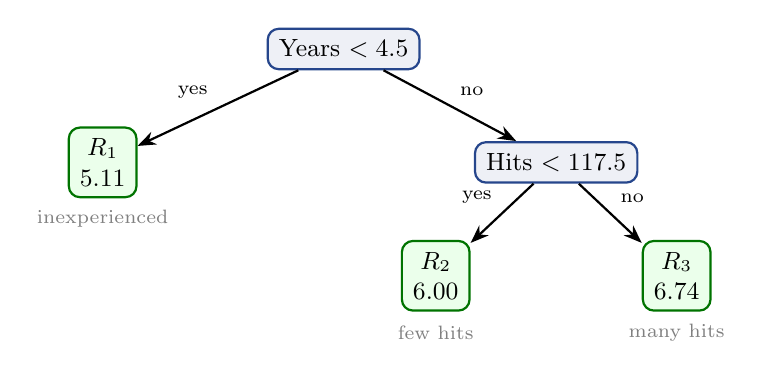
\begin{tikzpicture}[scale=0.9,
     >=Stealth,
     split/.style={draw=accent,fill=accent!8,rounded corners,thick,inner sep=4pt,align=center,font=\small},
     leaf/.style={draw=green!45!black,fill=green!8,rounded corners,thick,inner sep=4pt,align=center,font=\small},
     edg/.style={thick,->}]
    \node[split] (root) at (0,0)      {Years $<4.5$};
    \node[leaf]  (l1)   at (-3.4,-1.6){$R_1$\\ $5.11$};
    \node[split] (n2)   at (3.0,-1.6) {Hits $<117.5$};
    \node[leaf]  (l2)   at (1.3,-3.2) {$R_2$\\ $6.00$};
    \node[leaf]  (l3)   at (4.7,-3.2) {$R_3$\\ $6.74$};
    \draw[edg] (root) -- node[above left,font=\scriptsize]{yes} (l1);
    \draw[edg] (root) -- node[above right,font=\scriptsize]{no} (n2);
    \draw[edg] (n2)   -- node[above left,font=\scriptsize]{yes} (l2);
    \draw[edg] (n2)   -- node[above right,font=\scriptsize]{no} (l3);
    \node[font=\scriptsize,gray] at (-3.4,-2.4) {inexperienced};
    \node[font=\scriptsize,gray] at (1.3,-4.0) {few hits};
    \node[font=\scriptsize,gray] at (4.7,-4.0) {many hits};
  \end{tikzpicture}
  \end{center}
  \begin{takeaway}Each split is a yes/no question; each leaf reports the mean log-salary there. The highest earners sit in the deep right branch: experienced players with many hits.\end{takeaway}
\end{frame}

\begin{frame}{Hitters: how the tree partitions the data}
  \begin{center}
    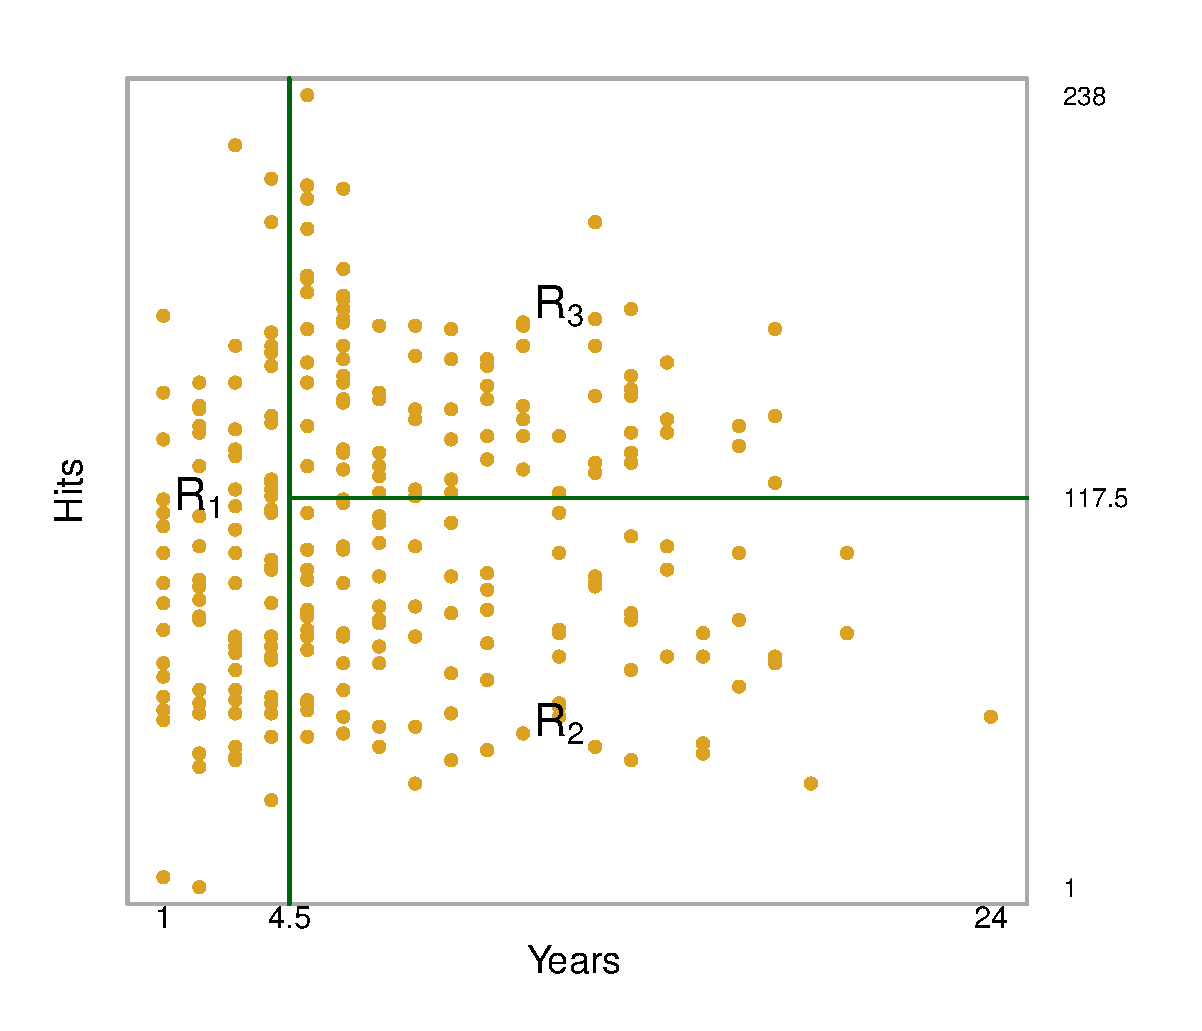
\includegraphics[width=0.62\textwidth,height=0.62\textheight,keepaspectratio]{8_2.pdf}
  \end{center}
  Each leaf is a rectangle in (Years, Hits).
  \islpsource{Figure 8.2}
\end{frame}

\begin{frame}{The same tree as a partition of predictor space}
  \begin{center}
  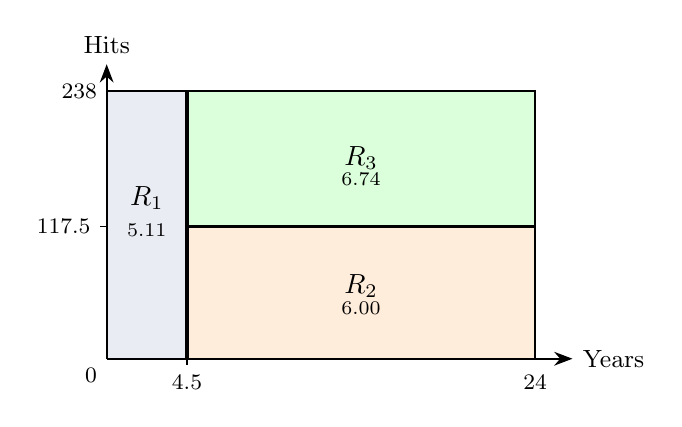
\begin{tikzpicture}[scale=0.68,>=Stealth,font=\small]
    % region fills
    \fill[accent!10] (0,0) rectangle (1.5,5);
    \fill[orange!14] (1.5,0) rectangle (8,2.47);
    \fill[green!14]  (1.5,2.47) rectangle (8,5);
    % partition lines
    \draw[very thick] (1.5,0) -- (1.5,5);
    \draw[very thick] (1.5,2.47) -- (8,2.47);
    % axes + frame
    \draw[->,thick] (0,0) -- (8.7,0) node[right]{Years};
    \draw[->,thick] (0,0) -- (0,5.5) node[above]{Hits};
    \draw (0,0) rectangle (8,5);
    % ticks
    \draw (1.5,0)--(1.5,-0.12) node[below,font=\footnotesize]{$4.5$};
    \node[below,font=\footnotesize] at (8,-0.12) {$24$};
    \draw (0,2.47)--(-0.12,2.47) node[left,font=\footnotesize]{$117.5$};
    \node[left,font=\footnotesize] at (0,5) {$238$};
    \node[below left,font=\footnotesize] at (0,0) {$0$};
    % region labels
    \node[font=\bfseries] at (0.75,3.0) {$R_1$};
    \node[font=\bfseries] at (4.75,1.35) {$R_2$};
    \node[font=\bfseries] at (4.75,3.75) {$R_3$};
    \node[font=\scriptsize] at (0.75,2.4) {5.11};
    \node[font=\scriptsize] at (4.75,0.95) {6.00};
    \node[font=\scriptsize] at (4.75,3.35) {6.74};
  \end{tikzpicture}
  \end{center}
  \begin{takeaway}$R_1$ holds inexperienced players; among experienced players, more hits ($R_3$) predicts higher salary than fewer ($R_2$).\end{takeaway}
\end{frame}

\begin{frame}{Why prune?}
  Recursive splitting with no stopping rule gives one leaf per training
  point --- zero training error, pathological test error.
  \begin{block}{Cost-complexity pruning}
    Choose a tree $T$ minimising:
    \[
      \sum_{j=1}^{|T|} \sum_{i \in R_j}(y_i - \bar y_{R_j})^2 + \alpha |T|.
    \]
  \end{block}
  \begin{readme}
    Here $|T|$ is the number of leaves and $\alpha\ge0$ the price paid
    per leaf: the first term rewards training fit, the $\alpha|T|$ term
    punishes size. Larger $\alpha$ $\Rightarrow$ smaller pruned tree;
    choose $\alpha$ by cross-validation.
  \end{readme}
\end{frame}

\begin{frame}{Classification trees: splitting rules}
  Same recursive splitting; predict majority class in each leaf.
  Two natural splitting criteria:
  \begin{block}{Gini and cross-entropy}
    \[
      G = \sum_k \hat p_{mk}(1 - \hat p_{mk}), \quad
      D = -\sum_k \hat p_{mk}\log \hat p_{mk}.
    \]
  \end{block}
  \begin{readme}[Reading the impurities]
    $\hat p_{mk}$ is the fraction of node-$m$ points in class $k$. Both
    $G$ and $D$ are \emph{small} when one class dominates ($\hat
    p_{mk}\!\approx\!1$) and \emph{large} at a 50/50 mix --- so a good
    split makes the child nodes as \emph{pure} as possible.
  \end{readme}
  \begin{takeaway}[Why not error rate?]
    The misclassification rate has many ties on small samples --- it
    splits poorly. Use Gini or cross-entropy for splitting; error rate
    for pruning.
  \end{takeaway}
\end{frame}

\begin{frame}{Trees vs.\ linear models: when each shines}
  \begin{center}
    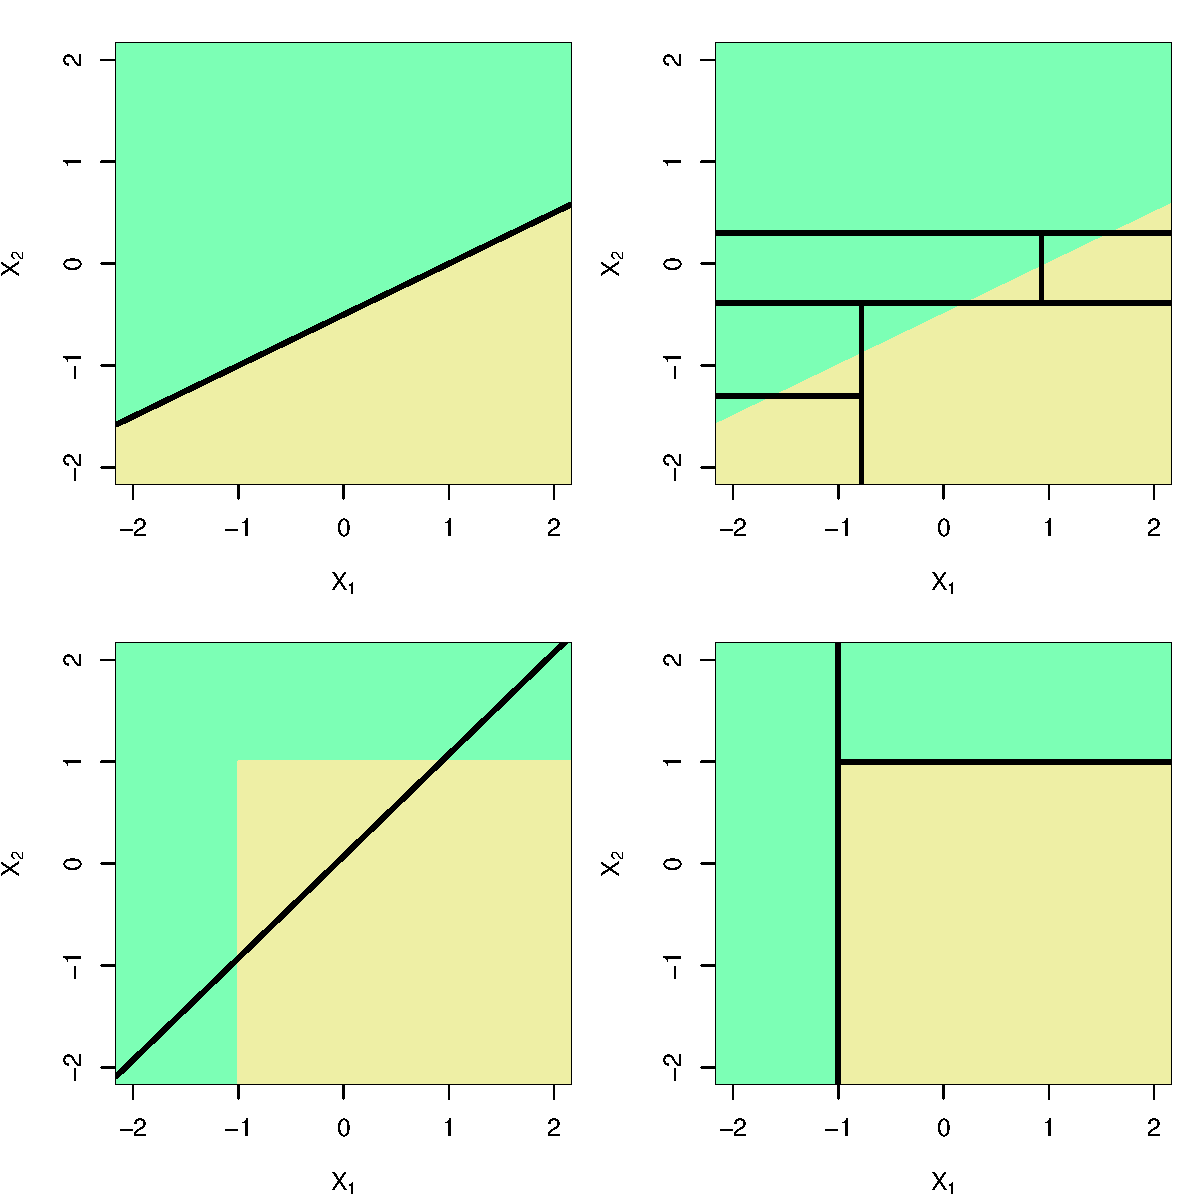
\includegraphics[width=0.92\textwidth,height=0.46\textheight,keepaspectratio]{8_7.pdf}
  \end{center}
  \begin{takeaway}Top: with a linear boundary the linear model wins and the tree's box-steps lose. Bottom: with non-linear, interacting structure the tree wins.\end{takeaway}
  \islpsource{Figure 8.7}
\end{frame}

\begin{frame}{Strengths and weaknesses of single trees}
  \begin{columns}[T]
    \begin{column}{0.48\textwidth}
      \textbf{Strengths}
      \begin{itemize}
        \item Easy to explain.
        \item Handle mixed and missing data.
        \item Capture interactions naturally.
        \item Robust to monotone transformations.
      \end{itemize}
    \end{column}
    \begin{column}{0.48\textwidth}
      \textbf{Weaknesses}
      \begin{itemize}
        \item Unstable: small data changes $\to$ very different trees.
        \item Predictions are step functions $\to$ rough.
        \item Often beaten by linear models on simple problems.
      \end{itemize}
    \end{column}
  \end{columns}
\end{frame}

% ====================== EXERCISES: Trees ======================
\begin{frame}{Exercise 8.1 --- Regression tree split by RSS [Math]}
\begin{exercise}
A regression tree is grown on this dataset:
\[
\begin{array}{c|cccccc}
x & 1 & 2 & 3 & 4 & 5 & 6\\\hline
y & 1.0 & 1.5 & 2.0 & 8.0 & 8.5 & 9.0
\end{array}
\]
\begin{enumerate}
  \item List the candidate split points (midpoints between consecutive $x$).
  \item Compute the total RSS for the splits $x<3.5$ and $x<2.5$.
  \item Which split is chosen? Give the predictions for $x=2$ and $x=5$.
  \item Predict $y$ for a new point $x=3.2$.
\end{enumerate}
\end{exercise}
\end{frame}

\begin{frame}{Solution --- Exercise 8.1 (1/2)}
\begin{solutionbox}
\textbf{(a) Candidate splits.} Any cutpoint between two consecutive $x$-values produces the same partition, so the midpoints are the canonical candidates: $s\in\{1.5,\,2.5,\,3.5,\,4.5,\,5.5\}$.

\medskip
\textbf{(b) RSS per split.} In each region the RSS-minimising constant prediction is the region \emph{mean}; the RSS adds the squared deviations from it.

\emph{Split $x<3.5$:} left $\{1.0,1.5,2.0\}$, mean $1.5$; right $\{8.0,8.5,9.0\}$, mean $8.5$.
\[ \mathrm{RSS}_L=(-0.5)^2+0^2+0.5^2=0.5,\quad \mathrm{RSS}_R=0.5,\quad \text{total}=1.0. \]

\emph{Split $x<2.5$:} left $\{1.0,1.5\}$, mean $1.25$; right $\{2.0,8.0,8.5,9.0\}$, mean $6.875$.
\[ \mathrm{RSS}_L=(-0.25)^2+0.25^2=0.125, \]
\[ \mathrm{RSS}_R=(-4.875)^2+1.125^2+1.625^2+2.125^2\approx 32.19,\quad \text{total}\approx 32.31. \]
\end{solutionbox}
\end{frame}

\begin{frame}{Solution --- Exercise 8.1 (2/2)}
\begin{solutionbox}
\textbf{(c) Chosen split and predictions.} The split $x<3.5$ gives total RSS $1.0$ versus $\approx32.31$ for $x<2.5$, so $x<3.5$ is chosen --- it separates the two tight $y$-clusters, whereas $x<2.5$ leaves the outlying $y=2.0$ stranded among the large values. Predictions are the leaf means: $x=2$ lands left $\Rightarrow \hat y=1.5$; $x=5$ lands right $\Rightarrow \hat y=8.5$.

\medskip
\textbf{(d) New point.} $x=3.2<3.5$, so it falls in the left region: $\hat y=1.5$.

\medskip
\emph{Interpretation:} a regression tree predicts a \emph{step function} --- every point in a leaf gets the same value, no matter how close it sits to the boundary.

\medskip
\textit{Common mistake:} interpolating between the two leaf means for a point near the cut (e.g.\ predicting $\approx5$ at $x=3.2$). Trees do not interpolate; the prediction jumps only when $x$ crosses $3.5$.
\end{solutionbox}
\end{frame}

\begin{frame}{Exercise 8.2 --- Gini index vs.\ classification error [Math]}
\begin{exercise}
A binary node contains $400$ positive and $400$ negative cases ($800$ total). Two candidate splits give:
\begin{itemize}
  \item \textbf{Split 1:} region A $(300+,100-)$ and region B $(100+,300-)$.
  \item \textbf{Split 2:} region A $(200+,400-)$ and region B $(200+,0-)$.
\end{itemize}
\begin{enumerate}
  \item Compute the weighted classification error for each split.
  \item Compute the weighted Gini index for each split.
  \item Which split does Gini prefer, and why is that desirable?
  \item Why are Gini / entropy preferred for \emph{growing} the tree?
\end{enumerate}
\end{exercise}
\end{frame}

\begin{frame}{Solution --- Exercise 8.2 (1/2)}
\begin{solutionbox}
\textbf{Set-up.} For a node with positive proportion $\hat p$: error $E=1-\max(\hat p,1-\hat p)$ (the fraction misclassified by the majority vote) and Gini $G=2\hat p(1-\hat p)$. A split is scored by the \emph{weighted} average of its two regions, each weighted by its share of the $800$ cases --- a large impure region must count more than a small one.

\medskip
\textbf{(a) Classification error.}
\emph{Split 1:} each region has $400$ cases with $\hat p=300/400=0.75$, so $E=1-0.75=0.25$ each; weighted:
\[ \tfrac{400}{800}(0.25)+\tfrac{400}{800}(0.25)=0.25. \]
\emph{Split 2:} region A ($600$ cases) is majority negative, $E=200/600=0.333$; region B ($200$ cases, pure) has $E=0$. Weighted:
\[ \tfrac{600}{800}(0.333)+\tfrac{200}{800}(0)=0.25. \]
Both splits give error $0.25$ --- the error criterion finds them \emph{indistinguishable}.
\end{solutionbox}
\end{frame}

\begin{frame}{Solution --- Exercise 8.2 (2/2)}
\begin{solutionbox}
\textbf{(b) Gini.}
\emph{Split 1:} each region $\hat p=0.75$, $G=2(0.75)(0.25)=0.375$; weighted $=0.375$.
\emph{Split 2:} region A $\hat p=200/600=1/3$, $G=2(\tfrac13)(\tfrac23)=0.444$, weight $0.75$; region B pure, $G=0$. Weighted $=0.75(0.444)+0.25(0)=0.333$.

\medskip
\textbf{(c)} Gini prefers \textbf{Split 2} ($0.333<0.375$) because it produces a \emph{pure} node (region B is all positive). Node purity is valuable even when it does not change the majority-vote error rate: a pure node needs no further splitting and yields confident predictions. Entropy behaves the same way.

\medskip
\textbf{(d)} Classification error is insensitive to node purity: it ignores improvements that do not flip the majority class. Gini and cross-entropy do reward purity, so they are used to \emph{grow} the tree; classification error is adequate when judging (or pruning toward) the final tree's accuracy.

\medskip
\textit{Common mistake:} averaging the two regions' impurities without their size weights --- with unequal regions (Split 2) the unweighted average is misleading.
\end{solutionbox}
\end{frame}

\begin{frame}{Exercise 8.3 --- Cost-complexity pruning [Concept]}
\begin{exercise}
Cost-complexity pruning selects a subtree $T\subset T_0$ minimising
\[ \sum_{m=1}^{|T|}\sum_{i:\,x_i\in R_m}(y_i-\hat y_{R_m})^2 \;+\; \alpha\,|T|. \]
\begin{enumerate}
  \item What do $|T|$ and $\alpha$ represent?
  \item What subtree results when $\alpha=0$, and when $\alpha\to\infty$?
  \item Why grow a large tree and then prune, rather than stop splitting early?
  \item How is $\alpha$ chosen?
\end{enumerate}
\end{exercise}
\end{frame}

\begin{frame}{Solution --- Exercise 8.3 (1/2)}
\begin{solutionbox}
\textbf{(a) The two ingredients.} $|T|$ is the number of terminal nodes (leaves) --- the natural measure of tree complexity, since each leaf is one fitted constant. $\alpha\ge 0$ is a tuning parameter: the \emph{price paid per leaf}. The criterion trades training fit (first term) against complexity ($\alpha|T|$), exactly as the lasso trades RSS against $\lambda\sum|\beta_j|$.

\medskip
\textbf{(b) The two extremes.} $\alpha=0$: leaves cost nothing, and every extra split can only lower the RSS term, so the full grown tree $T_0$ minimises the criterion. $\alpha\to\infty$: the penalty dominates, so the best subtree keeps as few leaves as possible --- the \emph{root alone}, a single node predicting the overall mean $\bar y$.

\medskip
\emph{Interpretation:} sliding $\alpha$ from $0$ to $\infty$ walks through a family of subtrees from most to least complex --- the tree analogue of a regularisation path.
\end{solutionbox}
\end{frame}

\begin{frame}{Solution --- Exercise 8.3 (2/2)}
\begin{solutionbox}
\textbf{(c) Why grow-then-prune beats early stopping.} Early stopping is short-sighted: a split that looks worthless now (tiny RSS reduction) may \emph{enable} a very valuable split just below it --- e.g.\ when two predictors matter only in combination, the first split shows little gain and a stopping rule would quit before the second, decisive split. Growing a large tree first and then pruning keeps such pairs, and cost-complexity pruning conveniently produces a \emph{nested sequence} of subtrees indexed by $\alpha$.

\medskip
\textbf{(d) Choosing $\alpha$.} By $K$-fold cross-validation: for a grid of $\alpha$ values, find the corresponding best subtree on each training fold, estimate its CV error, pick the $\alpha$ minimising CV error, then refit that subtree on the full data.

\medskip
\textit{Common mistake:} selecting $\alpha$ on the \emph{training} criterion --- the RSS term always favours the biggest tree, so training data alone would pick $\alpha=0$. Only held-out error can choose the penalty.
\end{solutionbox}
\end{frame}

% ====================== EXTENDED EXERCISE: Trees (regression) ======================
\begin{frame}{Extended Exercise 8.1 --- Grow a regression tree by hand [Math]}
\begin{longexercise}
Grow a regression tree on this data set (predictor $x$, response $y$):
\[
\begin{array}{c|cccccc}
x & 1 & 2 & 3 & 4 & 5 & 6\\\hline
y & 3 & 4 & 12 & 13 & 20 & 21
\end{array}
\]
\begin{enumerate}
  \item Give the root prediction and its RSS.
  \item Evaluate every candidate split (midpoints of consecutive $x$) and pick the one minimising total RSS.
  \item Split the resulting right child once more.
  \item State the final regions, their predictions, and the total RSS reduction.
\end{enumerate}
\end{longexercise}
\end{frame}

\begin{frame}{Solution --- Extended Exercise 8.1 (1/3)}
\begin{solutionbox}
\textbf{(a) Root.} Grand mean $\bar y=\frac{3+4+12+13+20+21}{6}=\frac{73}{6}\approx12.17$, and
\[ \mathrm{RSS}_{\text{root}}=\textstyle\sum y_i^2 - 6\bar y^2 = 1179-\tfrac{73^2}{6}\approx 290.83. \]

\textbf{(b) Candidate splits.} Predict each region by its mean; total RSS $=\mathrm{RSS}_L+\mathrm{RSS}_R$:
\[
\begin{array}{c|c|c}
\text{split} & \text{left}\mid\text{right mean} & \text{total RSS}\\\hline
x<1.5 & 3.0\mid14.0 & 190.0\\
x<2.5 & 3.5\mid16.5 & \mathbf{65.5}\\
x<3.5 & 6.33\mid18.0 & 86.7\\
x<4.5 & 8.0\mid20.5 & 82.5\\
x<5.5 & 10.4\mid21.0 & 197.2
\end{array}
\]
The split $x<2.5$ minimises RSS.
\end{solutionbox}
\end{frame}

\begin{frame}{Solution --- Extended Exercise 8.1 (2/3)}
\begin{solutionbox}
\textbf{First split $x<2.5$.} Left $\{3,4\}$ (mean $3.5$, RSS $0.5$); right $\{12,13,20,21\}$ (mean $16.5$, RSS $65$). The RSS drops from $290.83$ to $65.5$.

\medskip
\textbf{(c) Split the right child} $\{x\ge2.5\}=\{12,13,20,21\}$ at $x=3,4,5,6$:
\[
\begin{array}{c|c|c}
\text{split} & \text{left}\mid\text{right mean} & \text{child RSS}\\\hline
x<3.5 & 12.0\mid18.0 & 38.0\\
x<4.5 & 12.5\mid20.5 & \mathbf{1.0}\\
x<5.5 & 15.0\mid21.0 & 38.0
\end{array}
\]
The split $x<4.5$ wins, cutting the child's RSS from $65$ to $1.0$.

\medskip
\textit{Common mistake:} evaluating the second split on \emph{all six} points. Recursive splitting works within one node at a time --- only the right child's four points $\{12,13,20,21\}$ enter this computation.
\end{solutionbox}
\end{frame}

\begin{frame}{Solution --- Extended Exercise 8.1 (3/3)}
\begin{solutionbox}
\textbf{(d) Final tree (three leaves).}
\[
\begin{array}{c|c|c}
\text{region} & \text{rule} & \hat y\\\hline
R_1 & x<2.5 & 3.5\\
R_2 & 2.5\le x<4.5 & 12.5\\
R_3 & x\ge4.5 & 20.5
\end{array}
\]
Final total RSS $=0.5+0.5+0.5=1.5$.

\medskip
\textbf{Total RSS reduction.}
\[ 290.83 \;\xrightarrow{\text{split 1}}\; 65.5 \;\xrightarrow{\text{split 2}}\; 1.5, \]
a reduction of $290.83-1.5=\mathbf{289.33}$ ($225.33$ from the first split, $64.0$ from the second). The tree explains almost all variability because the data fall into three tight clusters.

\medskip
\emph{Why stop here:} each leaf's remaining RSS is only $0.5$; further splits would chase noise and cost-complexity pruning (any $\alpha>0.5$) would remove them again.
\end{solutionbox}
\end{frame}

% ====================== EXTENDED EXERCISE: Trees (classification) ======================
\begin{frame}{Extended Exercise 8.2 --- Impurity measures and pruning [Math]}
\begin{longexercise}
A binary-classification node holds $200$ cases: $100$ ``Yes'' and $100$ ``No''. Two candidate splits give:
\begin{itemize}
  \item \textbf{Split A:} $A_1=(80\text{ Yes},20\text{ No})$ and $A_2=(20\text{ Yes},80\text{ No})$.
  \item \textbf{Split B:} $B_1=(100\text{ Yes},40\text{ No})$ and $B_2=(0\text{ Yes},60\text{ No})$.
\end{itemize}
\begin{enumerate}
  \item For each split compute the weighted Gini index, cross-entropy and classification error.
  \item Which split wins under each criterion? Explain the disagreement.
  \item A pruned-tree sequence has subtrees with (leaves $|T|$, training errors $R$) $=(4,0),(3,4),(2,10),(1,40)$. For $\alpha\in\{0,5,20,50\}$ find the subtree minimising $R+\alpha|T|$.
\end{enumerate}
\end{longexercise}
\end{frame}

\begin{frame}{Solution --- Extended Exercise 8.2 (1/3)}
\begin{solutionbox}
For a node with ``Yes''-fraction $\hat p$:
\[ G=2\hat p(1-\hat p),\quad D=-\hat p\ln\hat p-(1-\hat p)\ln(1-\hat p),\quad E=1-\max(\hat p,1-\hat p), \]
and children are combined by their share of the $200$ cases.

\medskip
\textbf{Split A} ($A_1,A_2$ each $100$ cases, $\hat p=0.8$ and $0.2$ --- symmetric):
\[ G=2(0.8)(0.2)=0.32,\quad D=-0.8\ln0.8-0.2\ln0.2=0.500,\quad E=0.20. \]
Both children give identical values and equal weights $\tfrac{100}{200}=0.5$, so $G_A=0.32$, $D_A=0.500$, $E_A=0.20$.

\medskip
\emph{Note:} we use the natural log for $D$; switching to $\log_2$ rescales every entropy by the same factor and never changes which split wins.
\end{solutionbox}
\end{frame}

\begin{frame}{Solution --- Extended Exercise 8.2 (2/3)}
\begin{solutionbox}
\textbf{Split B.} $B_1$: $\hat p=100/140=0.714$, weight $0.7$; $B_2$ pure ($\hat p=0$), weight $0.3$.
\begin{align*}
G_B&=0.7\,[2(0.714)(0.286)]+0.3\,(0)=0.7(0.408)=\mathbf{0.286},\\
D_B&=0.7\,[-0.714\ln0.714-0.286\ln0.286]+0=0.7(0.598)=\mathbf{0.419},\\
E_B&=0.7\,(1-0.714)+0.3\,(0)=0.7(0.286)=\mathbf{0.20}.
\end{align*}

\medskip
\textbf{(2) Who wins?} Classification error ties ($E_A=E_B=0.20$) and cannot separate the splits. Gini ($0.286<0.32$) and entropy ($0.419<0.500$) both prefer \textbf{Split B}, because it carves out a \emph{pure} node $B_2$. Purity is rewarded by Gini/entropy even when majority-vote error is unchanged --- which is why we \emph{grow} trees with Gini or entropy, not error.
\end{solutionbox}
\end{frame}

\begin{frame}{Solution --- Extended Exercise 8.2 (3/3)}
\begin{solutionbox}
\textbf{(3) Cost-complexity pruning.} Minimise $R_\alpha(T)=R(T)+\alpha|T|$ over the nested subtrees:
\[
\begin{array}{c|cccc}
 & (4,0) & (3,4) & (2,10) & (1,40)\\\hline
\alpha{=}0 & \mathbf{0} & 4 & 10 & 40\\
\alpha{=}5 & 20 & \mathbf{19} & 20 & 45\\
\alpha{=}20 & 80 & 64 & \mathbf{50} & 60\\
\alpha{=}50 & 200 & 154 & 110 & \mathbf{90}
\end{array}
\]
Winners: $\alpha{=}0\!\to\!4$ leaves, $\alpha{=}5\!\to\!3$ leaves, $\alpha{=}20\!\to\!2$ leaves, $\alpha{=}50\!\to\!$ the root. As $\alpha$ grows the optimal subtree shrinks (breakpoints at $\alpha=4,6,30$) --- the nested ``weakest-link'' sequence that cross-validation then searches over.

\medskip
\emph{Sample entry:} for $\alpha=5$ and the $3$-leaf tree, $R_\alpha=R+\alpha|T|=4+5\cdot3=19$ --- the smallest value in its row, so $3$ leaves win at that price.
\end{solutionbox}
\end{frame}



% ============================================================
\section{Bagging / RF}
% ============================================================

\begin{frame}{Bagging: variance reduction by averaging}
  \begin{block}{Algorithm}
    \begin{enumerate}
      \item Draw $B$ bootstrap samples of size $n$.
      \item Fit a deep tree to each sample.
      \item Average $B$ predictions (regression) or majority-vote
            (classification).
    \end{enumerate}
  \end{block}
  \begin{takeaway}[Free benefits]
    \begin{itemize}
      \item Variance reduction via averaging --- bias unchanged.
      \item OOB error: each training point appears in $\sim 63\,\%$
            of the bootstrap samples; the held-out $37\,\%$ act as
            built-in CV.
      \item No tuning required.
    \end{itemize}
  \end{takeaway}
\end{frame}

\begin{frame}{Out-of-bag: the leftover third is a free test set}
  \begin{center}
  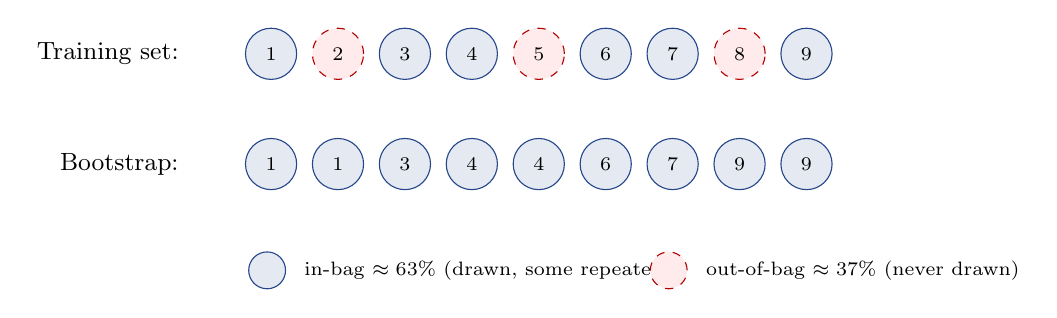
\begin{tikzpicture}[>=Stealth,font=\footnotesize,
     ib/.style={circle,draw=accent,fill=accent!12,minimum size=6.5mm,inner sep=0pt,font=\scriptsize},
     ob/.style={circle,draw=red!70!black,dashed,fill=red!8,minimum size=6.5mm,inner sep=0pt,font=\scriptsize}]
    \node[anchor=east,font=\small] at (0.5,2.2) {Training set:};
    \foreach \i/\c in {1/ib,2/ob,3/ib,4/ib,5/ob,6/ib,7/ib,8/ob,9/ib}
      \node[\c] at (0.7+\i*0.85,2.2) {\i};
    \node[anchor=east,font=\small] at (0.5,0.8) {Bootstrap:};
    \foreach \k/\v in {1/1,2/1,3/3,4/4,5/4,6/6,7/7,8/9,9/9}
      \node[ib] at (0.7+\k*0.85,0.8) {\v};
    \node[ib,scale=0.72] at (1.5,-0.55) {};
    \node[anchor=west,font=\scriptsize] at (1.85,-0.55){in-bag $\approx 63\%$ (drawn, some repeated)};
    \node[ob,scale=0.72] at (6.6,-0.55) {};
    \node[anchor=west,font=\scriptsize] at (6.95,-0.55){out-of-bag $\approx 37\%$ (never drawn)};
  \end{tikzpicture}
  \end{center}
  \begin{takeaway}A bootstrap draw of $n$ points with replacement repeats some (in-bag) and misses others: $\big(1-\tfrac1n\big)^{n}\!\to e^{-1}\!\approx\!0.37$. Scoring each point with only the trees that did \emph{not} see it gives the OOB error --- built-in cross-validation, for free.\end{takeaway}
\end{frame}

\begin{frame}{Why averaging helps: one deep tree vs.\ a bagged hundred}
  \begin{center}
\includegraphics[width=0.88\textwidth,height=0.56\textheight,keepaspectratio]{ch08_x_bagging_variance.png}\end{center}
  \begin{takeaway}On simulated $y=\sin(2x)+\varepsilon$ a single deep tree is a jagged step function (MSE vs.\ truth $0.15$); averaging $100$ bootstrap trees smooths it to MSE $0.07$ --- bagging averages away single-tree variance while the bias stays put.\end{takeaway}
\end{frame}

\begin{frame}{Random forests: the de-correlation trick}
  Bagging averages \emph{correlated} trees because the same strong
  predictor tends to dominate the top split.
  \begin{block}{Key idea}
    At each split, consider only $m$ randomly chosen predictors out of
    $p$.
  \end{block}
  \begin{readme}[Default values of $m$]
    \begin{itemize}
      \item Classification: $m = \sqrt{p}$.
      \item Regression: $m = p / 3$.
    \end{itemize}
  \end{readme}
  \begin{takeaway}
    Forcing different trees to use different predictors lowers their
    pairwise correlation, which makes the average more effective.
    With $m = p$ random forests reduce to bagging.
  \end{takeaway}
\end{frame}

\begin{frame}{Random forest: error vs.\ number of trees}
  \begin{center}
    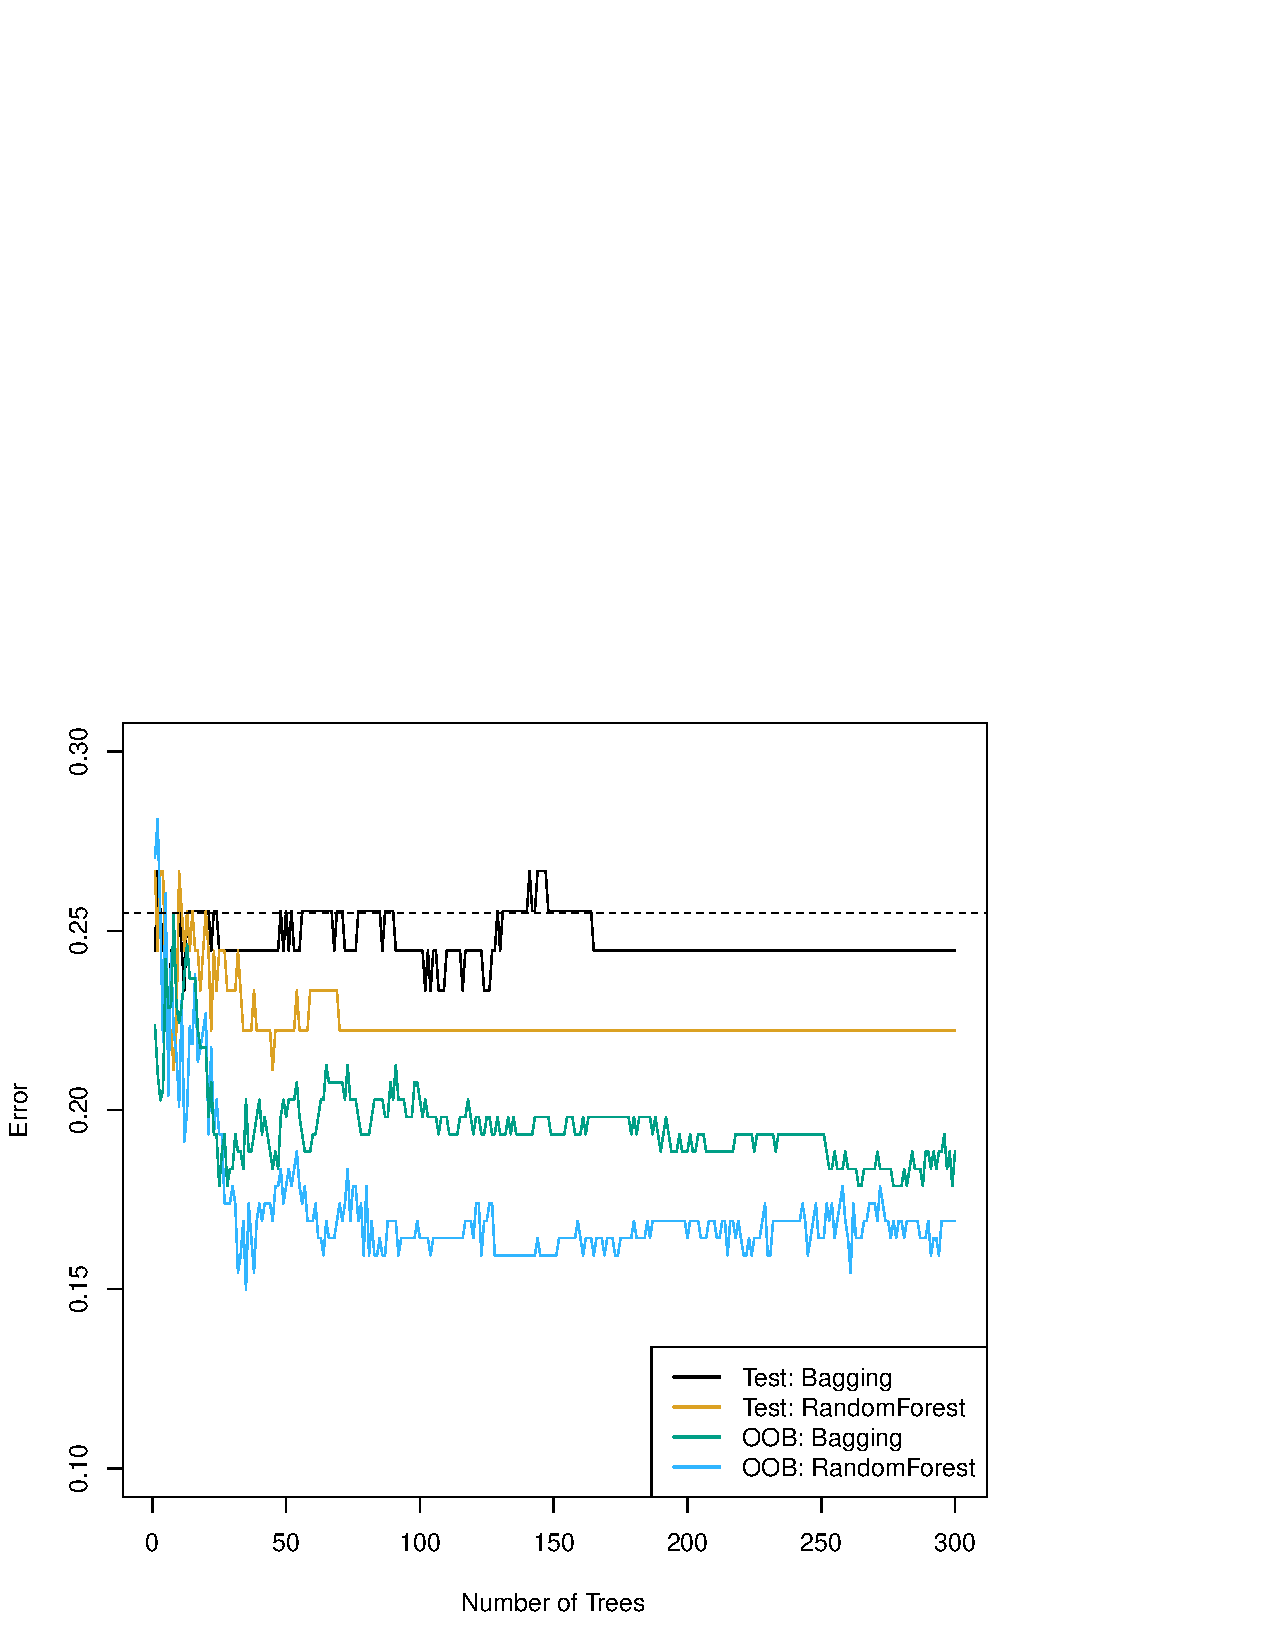
\includegraphics[width=0.85\textwidth,height=0.50\textheight,keepaspectratio]{8_8.pdf}
  \end{center}
  \begin{takeaway}Test error falls then flattens after a few hundred trees. More trees never hurt --- unlike boosting, you cannot ``overfit'' a forest by growing it larger, only hit diminishing returns.\end{takeaway}
  \islpsource{Figure 8.8}
\end{frame}

\begin{frame}{Test error vs.\ ensemble size: bagging, forest, boosting}
  \begin{center}
    
\includegraphics[width=0.68\textwidth,height=0.55\textheight,keepaspectratio]{ch08_ensemble_error.png}
  \end{center}
  \begin{takeaway}All three ensembles beat a single tree. Bagging and the forest fall fast then flatten; slow-learning boosting starts higher but reaches the lowest test MSE.\end{takeaway}
\end{frame}

\begin{frame}{Variable importance in random forests}
  \begin{block}{Two notions}
    \begin{itemize}
      \item \textbf{Impurity importance}: total decrease in node
            impurity due to splits on $X_j$, summed across trees.
      \item \textbf{Permutation importance}: shuffle $X_j$ in OOB
            samples and measure the increase in error.
    \end{itemize}
  \end{block}
  \begin{alertblock}{Caveat}
    Correlated predictors share importance --- you may need to
    interpret pairs together.
  \end{alertblock}
\end{frame}

\begin{frame}{Variable importance on the Boston data}
  \begin{center}
    
\includegraphics[width=0.72\textwidth,height=0.60\textheight,keepaspectratio]{ch08_importance.png}
  \end{center}
  \begin{takeaway}Two predictors dominate: \texttt{lstat} (\% lower-status population) and \texttt{rm} (average rooms). Housing value is driven mostly by neighbourhood status and dwelling size; the rest contribute little.\end{takeaway}
\end{frame}


\begin{frame}{Mini-check: trees and ensembles}
  \begin{readme}[Quick self-assessment]
    \begin{enumerate}
      \item Why is a single tree typically high-variance?
      \item Why does feature subsampling at each split improve random
            forests over plain bagging?
      \item Can you ``overfit'' a random forest by growing too many
            trees?
    \end{enumerate}
  \end{readme}
  \begin{takeaway}[Answers]
    1.\ Greedy splits, no shrinkage, perfectly fit training data.\quad
    2.\ Decorrelates the trees, so averaging is more effective.\quad
    3.\ No --- adding more trees never hurts, you just hit diminishing
        returns.
  \end{takeaway}
\end{frame}

% ====================== EXERCISES: Bagging / RF ======================
\begin{frame}{Exercise 8.4 --- Bagging and OOB error [Concept]}
\begin{exercise}
\begin{enumerate}
  \item If each tree has variance $\sigma^2$, what is the variance of the average of $B$ trees when they are independent? When they have pairwise correlation $\rho$?
  \item What fraction of observations are out-of-bag (OOB) for a given bootstrap tree? Derive it.
  \item What does the OOB error estimate, and why is it almost free?
\end{enumerate}
\end{exercise}
\end{frame}

\begin{frame}{Solution --- Exercise 8.4 (1/2)}
\begin{solutionbox}
\textbf{(a) Variance of the average.} For the mean of $B$ trees, expand the variance of a sum ($B$ variance terms, $B(B-1)$ covariance terms $\rho\sigma^2$):
\[ \operatorname{Var}\!\Big(\tfrac1B\sum_b \hat f_b\Big)=\frac{1}{B^2}\Big[B\sigma^2+B(B-1)\rho\sigma^2\Big]
=\rho\sigma^2+\frac{1-\rho}{B}\,\sigma^2. \]
\emph{Independent trees} ($\rho=0$): $\operatorname{Var}=\sigma^2/B\to0$ --- averaging could remove \emph{all} variance. \emph{Correlated trees:}
\[ \rho\sigma^2+\frac{1-\rho}{B}\sigma^2 \;\xrightarrow{B\to\infty}\; \rho\sigma^2. \]
\emph{Interpretation:} bagging drives the second term to zero for free (more trees), but the floor $\rho\sigma^2$ remains --- the correlation between trees caps how much variance averaging can remove. This is exactly the lever random forests attack.
\end{solutionbox}
\end{frame}

\begin{frame}{Solution --- Exercise 8.4 (2/2)}
\begin{solutionbox}
\textbf{(b) OOB fraction.} A bootstrap sample makes $n$ independent draws \emph{with replacement}; each draw misses observation $i$ with probability $1-\tfrac1n$, so
\[ \Pr(i\ \text{never drawn})=\Big(1-\tfrac1n\Big)^{n}\;\xrightarrow{n\to\infty}\; e^{-1}\approx 0.368 \]
(already $0.366$ at $n=100$). So about $1/3$ of observations are OOB and $2/3$ in-bag for each tree.

\medskip
\textbf{(c) OOB error.} Each observation is OOB for roughly $B/3$ of the trees; predicting it using \emph{only those} trees gives an honest held-out prediction. Aggregating over all $n$ observations yields the OOB error, which approximates the test / CV error --- and it comes free with a single fit, since it reuses trees that were grown anyway.

\medskip
\textit{Common mistake:} scoring OOB points with \emph{all} $B$ trees. Trees that saw the point in-bag have memorised it, so including them makes the error estimate optimistically low.
\end{solutionbox}
\end{frame}

\begin{frame}{Exercise 8.5 --- Random forests and decorrelation [Concept/Math]}
\begin{exercise}
\begin{enumerate}
  \item How does a random forest differ from bagging? What is $m$?
  \item Give the usual choice of $m$ for classification and for regression with $p$ predictors.
  \item Using the variance formula $\rho\sigma^2+\frac{1-\rho}{B}\sigma^2$, explain why restricting to $m$ predictors helps.
  \item With $p=16$, what is $m$ for classification and for regression?
\end{enumerate}
\end{exercise}
\end{frame}

\begin{frame}{Solution --- Exercise 8.5 (1/2)}
\begin{solutionbox}
\textbf{(a) The difference.} A random forest is bagging plus a twist: at \emph{each split} only a random subset of $m$ of the $p$ predictors is considered as candidates. The subset is redrawn \emph{at every split}, not once per tree, so a single tree can still use all predictors --- just never all at the same decision. Bagging is the special case $m=p$.

\medskip
\textbf{(b) Default values.} Classification: $m\approx\sqrt{p}$. Regression: $m\approx p/3$. These are rules of thumb --- $m$ is a tuning parameter worth checking by OOB error or CV.

\medskip
\emph{Interpretation:} $m$ is the decorrelation dial: $m=p$ recovers bagging, small $m$ forces diverse trees.
\end{solutionbox}
\end{frame}

\begin{frame}{Solution --- Exercise 8.5 (2/2)}
\begin{solutionbox}
\textbf{(c) Why restricting to $m$ predictors helps.} If one or two predictors are very strong, in bagging almost every bootstrap tree splits on them at the top, so the trees look alike --- $\rho$ is large and the limiting variance $\rho\sigma^2$ stays high, no matter how big $B$ is. With $m<p$ a split ignores each given predictor with probability $(p-m)/p$ --- e.g.\ $m=4$ of $p=16$ hides the dominant predictor at $12/16=75\,\%$ of splits --- so trees are forced to differ. That lowers $\rho$, hence the floor $\rho\sigma^2$, and averaging becomes far more effective.

\medskip
\textbf{(d) With $p=16$:} classification $m=\sqrt{16}=4$; regression $m=16/3\approx 5$ (round $5.33$ down to an integer).

\medskip
\textit{Common mistake:} expecting small $m$ to reduce \emph{bias}. Restricting candidates slightly \emph{raises} each tree's bias; the payoff is purely in decorrelation, i.e.\ variance reduction of the average.
\end{solutionbox}
\end{frame}


% ============================================================
\section{Boosting}
% ============================================================

\begin{frame}{Boosting: idea}
  Boosting builds a sequence of weak trees, each fitted to the
  residuals of the previous fit. Slow, careful adaptation.
  \begin{block}{Gradient-boosting algorithm}
    \begin{enumerate}
      \item Initialise $\hat f(x) = 0$, $r_i = y_i$.
      \item For $b = 1, \ldots, B$:
        \begin{enumerate}
          \item Fit a tree $\hat f^b$ with $d$ splits to $(x_i, r_i)$.
          \item Update $\hat f \leftarrow \hat f + \nu \hat f^b$.
          \item Update residuals
                $r_i \leftarrow r_i - \nu \hat f^b(x_i)$.
        \end{enumerate}
    \end{enumerate}
  \end{block}
\end{frame}

\begin{frame}{Boosting: each tree fits what the last one missed}
  \begin{center}
  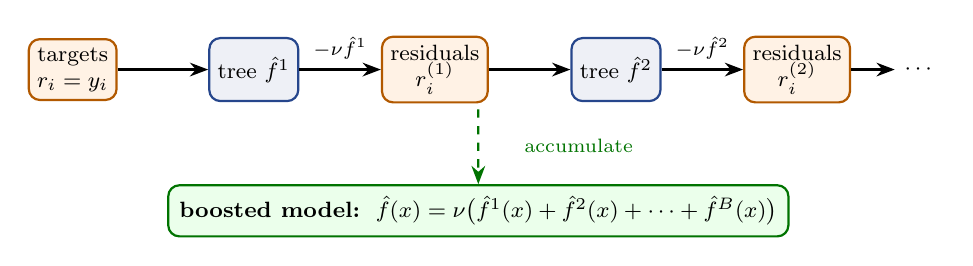
\begin{tikzpicture}[scale=0.92,>=Stealth,font=\footnotesize,
     tb/.style={draw=accent,fill=accent!8,rounded corners,thick,inner sep=3pt,align=center,minimum height=8mm},
     rb/.style={draw=orange!70!black,fill=orange!10,rounded corners,thick,inner sep=3pt,align=center},
     ar/.style={->,thick}]
    \node[rb] (r0) at (0,0)   {targets\\ $r_i=y_i$};
    \node[tb] (t1) at (2.5,0) {tree $\hat f^1$};
    \node[rb] (r1) at (5.0,0) {residuals\\ $r_i^{(1)}$};
    \node[tb] (t2) at (7.5,0) {tree $\hat f^2$};
    \node[rb] (r2) at (10.0,0){residuals\\ $r_i^{(2)}$};
    \node (dots) at (11.7,0) {$\cdots$};
    \draw[ar] (r0)--(t1);
    \draw[ar] (t1)--node[above,font=\scriptsize]{$-\nu\hat f^1$}(r1);
    \draw[ar] (r1)--(t2);
    \draw[ar] (t2)--node[above,font=\scriptsize]{$-\nu\hat f^2$}(r2);
    \draw[ar] (r2)--(dots);
    \node[draw=green!45!black,fill=green!8,rounded corners,thick,inner sep=4pt,align=center] (sum) at (5.6,-1.95)
      {\textbf{boosted model:}\ \ $\hat f(x)=\nu\big(\hat f^1(x)+\hat f^2(x)+\cdots+\hat f^B(x)\big)$};
    \draw[ar,green!45!black,dashed] (5.6,-0.55)--(sum.north);
    \node[green!45!black,font=\scriptsize,anchor=west] at (6.1,-1.05){accumulate};
  \end{tikzpicture}
  \end{center}
  \begin{readme}[Reading the update]
    Fit a small tree to the current \emph{residuals} $r_i$ (what the
    model still gets wrong), add only a fraction $\nu$ of it
    ($0{<}\nu{\ll}1$), then shrink the residuals. Small $\nu$ = slow,
    cautious learning; the depth $d$ caps the interaction order.
  \end{readme}
\end{frame}

\begin{frame}{Boosting tuning parameters}
  \begin{readme}[The trio]
    \begin{itemize}
      \item $B$ --- number of trees. Too large $\Rightarrow$
            overfitting.
      \item $\nu$ --- learning rate (typically $0.001$ to $0.1$).
      \item $d$ --- tree depth (often $d = 1$ or $2$ suffices).
    \end{itemize}
  \end{readme}
  \begin{takeaway}[Trade-off]
    Smaller $\nu$ usually wins but requires larger $B$. The product
    $\nu \cdot B$ controls effective fitting effort. Choose all three
    by CV.
  \end{takeaway}
\end{frame}

\begin{frame}{Boosting vs.\ random forest: head-to-head}
  \begin{center}
    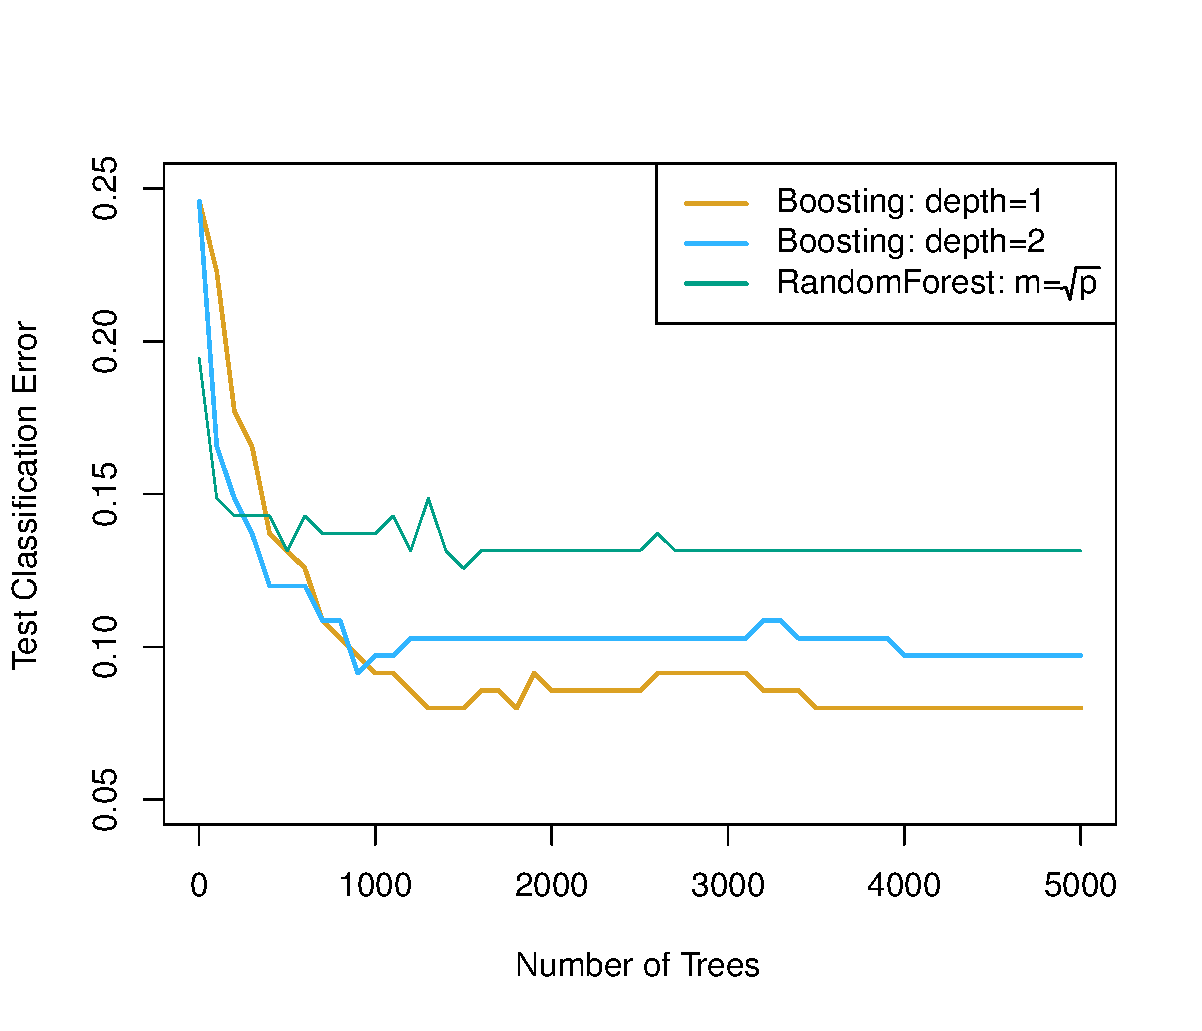
\includegraphics[width=0.85\textwidth,height=0.50\textheight,keepaspectratio]{8_11.pdf}
  \end{center}
  \begin{takeaway}With enough trees and a small learning rate, boosting often edges out the random forest on test error --- but it must be tuned carefully, whereas the forest is strong out of the box.\end{takeaway}
  \islpsource{Figure 8.11}
\end{frame}

\begin{frame}{Modern boosting libraries}
  Industrial implementations dominate Kaggle on tabular data.
  \begin{block}{The big three}
    \texttt{XGBoost}, \texttt{LightGBM}, \texttt{CatBoost}.
  \end{block}
  \begin{readme}[Beyond textbook gradient boosting]
    Feature subsampling, second-order gradients, $\ell_1$ / $\ell_2$
    regularisation on leaf weights, GPU support, native categorical
    handling, histogram-based splits.
  \end{readme}
\end{frame}

\begin{frame}{BART: Bayesian Additive Regression Trees}
  \begin{block}{Idea}
    A sum of $K$ small trees (each a ``weak learner''), updated one
    tree at a time using a Bayesian posterior-style move.
  \end{block}
  \begin{takeaway}
    Combines flavours of bagging (averaging) and boosting (sequential
    update). Out-of-the-box hyperparameters often work; the Bayesian
    framework gives credible intervals for free. Implementations:
    \texttt{ISLP.bart}, \texttt{PyMC}.
  \end{takeaway}
\end{frame}

% ====================== EXERCISE: Boosting ======================
\begin{frame}{Exercise 8.6 --- Boosting tuning parameters [Concept]}
\begin{exercise}
Gradient boosting with regression trees has three tuning parameters.
\begin{enumerate}
  \item Name them and state what each controls.
  \item What does ``slow learning'' mean and why does it help?
  \item How do $B$ and $\lambda$ interact, and what is the danger of a large $B$?
  \item What does $d$ control? What model do we get when $d=1$?
\end{enumerate}
\end{exercise}
\end{frame}

\begin{frame}{Solution --- Exercise 8.6 (1/2)}
\begin{solutionbox}
\textbf{(a) The three parameters.} $B$ = number of trees (how many boosting rounds); $\lambda$ = shrinkage / learning rate (typically $0.01$ or $0.001$) --- the fraction of each new tree actually added; $d$ = number of splits per tree (interaction depth / tree size).

\medskip
\textbf{(b) Slow learning.} Each new tree is fitted to the current \emph{residuals} --- what the ensemble still gets wrong --- but only $\lambda$ times its prediction is added:
\[ \hat f(x)\leftarrow\hat f(x)+\lambda\,\hat f^{\,b}(x),\qquad r_i\leftarrow r_i-\lambda\,\hat f^{\,b}(x_i). \]
With small $\lambda$ no single tree can dominate; the ensemble creeps toward the signal in many tiny, mutually correcting steps rather than a few large ones. This shrinkage reduces overfitting and improves generalisation --- the same logic as ridge/lasso shrinkage, applied to trees.
\end{solutionbox}
\end{frame}

\begin{frame}{Solution --- Exercise 8.6 (2/2)}
\begin{solutionbox}
\textbf{(c) How $B$ and $\lambda$ interact.} A smaller $\lambda$ requires a larger $B$ to reach the same total fitting effort (roughly, effort $\propto \lambda\cdot B$) --- they trade off. The danger: unlike random forests, boosting keeps re-fitting the residuals, so with $B$ too large it starts fitting \emph{noise} --- it \emph{can} overfit. Choose $B$ by cross-validation or early stopping on a validation set.

\medskip
\textbf{(d) The role of $d$.} $d$ caps how many variables can interact along one tree's path, i.e.\ the \emph{interaction order}. $d=1$ gives stumps: each tree involves a single predictor, so the boosted model is purely \emph{additive} --- a tree-built cousin of a GAM. Larger $d$ allows higher-order interactions among predictors.

\medskip
\textit{Common mistake:} tuning $B$ by training error --- it decreases monotonically in $B$, so it never signals when to stop; only validation/CV error turns upward.
\end{solutionbox}
\end{frame}



% ============================================================
\section{Python Lab}

\begin{frame}{Python lab --- run it live in the notebook}
  \begin{labnote}[Companion notebook: \texttt{chapter\_08\_lab.ipynb}]
    The code in this section is meant to be \textbf{demonstrated live}. Open the companion Jupyter notebook and run it cell by cell:
    \begin{itemize}
      \item a single regression tree and cost-complexity pruning;
      \item random forests and gradient boosting;
      \item an optional XGBoost comparison.
    \end{itemize}
    Data loads via the \texttt{ISLP} package or the bundled CSV files; the notebook ends with hands-on exercises.
  \end{labnote}
\end{frame}


% ============================================================

\begin{frame}[fragile]{Decision tree on Carseats}
  \begin{lstlisting}[basicstyle=\ttfamily\scriptsize]
from sklearn.tree import DecisionTreeRegressor, plot_tree
from sklearn.model_selection import train_test_split
from ISLP import load_data

Carseats = load_data("Carseats")  # load data
X = pd.get_dummies(Carseats.drop(columns="Sales"), drop_first=True)  # dummy-code factors
y = Carseats["Sales"]  # response

Xtr, Xte, ytr, yte = train_test_split(X, y, test_size=0.3, random_state=0)  # 70/30 split
tree = DecisionTreeRegressor(max_depth=4).fit(Xtr, ytr)  # grow a depth-4 tree
plot_tree(tree, feature_names=X.columns, filled=True, fontsize=7)  # draw fitted tree
  \end{lstlisting}
\end{frame}

\begin{frame}[fragile]{Random forest}
  \begin{lstlisting}[basicstyle=\ttfamily\scriptsize]
from sklearn.ensemble import RandomForestRegressor
import numpy as np

rf = RandomForestRegressor(n_estimators=500, max_features="sqrt",  # B=500, m=sqrt(p)
                            random_state=0, oob_score=True).fit(Xtr, ytr)  # keep OOB score
print("OOB R^2:", rf.oob_score_)  # OOB error: free validation
print("Test MSE:", ((yte - rf.predict(Xte))**2).mean())  # held-out test error

imp = pd.Series(rf.feature_importances_, index=X.columns)  # impurity importances
imp.sort_values().plot.barh()  # importance plot
  \end{lstlisting}
\end{frame}

\begin{frame}[fragile]{Gradient boosting and XGBoost}
  \begin{lstlisting}[basicstyle=\ttfamily\scriptsize]
from sklearn.ensemble import GradientBoostingRegressor
gb = GradientBoostingRegressor(n_estimators=1000, learning_rate=0.01,  # B=1000, lambda=0.01
                               max_depth=3, random_state=0).fit(Xtr, ytr)  # depth d=3
print("Test MSE:", ((yte - gb.predict(Xte))**2).mean())  # boosted test error

# Optional XGBoost
import xgboost as xgb
bst = xgb.XGBRegressor(n_estimators=2000, learning_rate=0.05,  # more trees, larger step
                       max_depth=4, subsample=0.8).fit(Xtr, ytr)  # row subsampling
  \end{lstlisting}
\end{frame}

% ====================== EXERCISE: Python (Boston) ======================
\begin{frame}[fragile]{Exercise 8.7 --- Random forest \& boosting on Boston [Python]}
\begin{exercise}
Using \texttt{Boston.csv} (target \texttt{medv}):
\begin{enumerate}
  \item Fit a random forest and a gradient-boosting regressor; report test MSE.
  \item Read off the most important features from the random forest.
  \item Interpret the result.
\end{enumerate}
\end{exercise}
\end{frame}

\begin{frame}[fragile]{Solution --- Exercise 8.7 (1/3)}
\begin{solutionbox}
\begin{lstlisting}
import pandas as pd
from sklearn.ensemble import (RandomForestRegressor,
                              GradientBoostingRegressor)
from sklearn.model_selection import train_test_split
from sklearn.metrics import mean_squared_error

Boston = pd.read_csv('../../ALL CSV FILES - 2nd Edition/Boston.csv')
Boston = Boston.drop(columns=[c for c in ['Unnamed: 0']  # drop index col
                              if c in Boston.columns])
X = Boston.drop(columns='medv'); y = Boston['medv']  # target: medv
Xtr, Xte, ytr, yte = train_test_split(X, y, test_size=0.3,  # 70/30 split
                                      random_state=0)
\end{lstlisting}
\emph{Set-up:} we hold out $30\,\%$ as a test set; fixing \texttt{random\_state} makes the split (and every number below) reproducible.
\end{solutionbox}
\end{frame}

\begin{frame}[fragile]{Solution --- Exercise 8.7 (2/3)}
\begin{solutionbox}
\begin{lstlisting}[basicstyle=\ttfamily\scriptsize]
rf = RandomForestRegressor(n_estimators=500, max_features='sqrt',  # 500 trees, m=sqrt(p)
                           random_state=0).fit(Xtr, ytr)  # fit on training set
print('RF  test MSE:', mean_squared_error(yte, rf.predict(Xte)))  # held-out error

gb = GradientBoostingRegressor(n_estimators=1000, learning_rate=0.01,  # slow learning
                               max_depth=3, random_state=0).fit(Xtr, ytr)  # depth 3
print('GBM test MSE:', mean_squared_error(yte, gb.predict(Xte)))  # compare with RF

imp = pd.Series(rf.feature_importances_,  # impurity importances
                index=X.columns).sort_values(ascending=False)  # largest first
print(imp.head())  # top predictors
\end{lstlisting}
\emph{What it prints (this seed):} RF test MSE $\approx19.6$, boosting $\approx13.5$ --- versus $\approx27$ for a single unpruned tree on the same split. The importance list is headed by \texttt{lstat} ($\approx0.28$) and \texttt{rm} ($\approx0.27$).
\end{solutionbox}
\end{frame}

\begin{frame}{Solution --- Exercise 8.7 (3/3)}
\begin{solutionbox}
\textbf{Interpretation.} Both ensembles reach a test MSE well below a single tree (typically around $10$--$15$ for Boston). On this particular split the $m=\sqrt p$ forest lands higher ($\approx19.6$) while boosting reaches $\approx13.5$: Boston has a few dominant predictors, so restricting each split to $\sqrt{12}\approx3$ candidates costs accuracy here --- Extended Exercise 8.3 shows that a larger $m$ closes the gap.

\medskip
The importance ranking is dominated by \texttt{lstat} (\% lower-status population) and \texttt{rm} (average number of rooms): housing value depends most on socio-economic status and dwelling size. Importances measure the total RSS reduction attributable to each variable summed across all trees, normalised to sum to $1$.

\medskip
\textit{Common mistake:} comparing models fitted or evaluated on \emph{different} splits --- always fix one train/test split (or use CV) before declaring a winner, and remember that single-split MSEs carry noticeable seed-to-seed noise.
\end{solutionbox}
\end{frame}

% ====================== EXTENDED EXERCISE: Python (Boston) ======================
\begin{frame}{Extended Exercise 8.3 --- Bagging vs.\ forest vs.\ boosting [Python]}
\begin{longexercise}
Using \texttt{Boston.csv} (target \texttt{medv}), fit and compare three ensembles against a single tree:
\begin{enumerate}
  \item \textbf{Bagging} (a forest that considers all $p$ predictors at each split);
  \item a \textbf{random forest}, tuning $m=$ features tried per split;
  \item \textbf{gradient boosting}, tuning $(B,\lambda,d)=$ (trees, learning rate, depth).
\end{enumerate}
Report the test MSE of each, and read off the random-forest variable-importance ranking. Which method wins, and which predictors matter?
\end{longexercise}
\end{frame}

\begin{frame}[fragile]{Solution --- Extended Exercise 8.3 (1/3)}
\begin{solutionbox}
\textbf{Load the data; fit a single tree and bagging} (\texttt{max\_features=p} $=$ bagging).
\begin{lstlisting}[basicstyle=\ttfamily\scriptsize]
import pandas as pd
from sklearn.model_selection import train_test_split
from sklearn.tree import DecisionTreeRegressor
from sklearn.ensemble import RandomForestRegressor, GradientBoostingRegressor
from sklearn.metrics import mean_squared_error as mse
B = pd.read_csv('../../ALL CSV FILES - 2nd Edition/Boston.csv')  # load
B = B.drop(columns=[c for c in ['Unnamed: 0', ''] if c in B.columns])
X, y = B.drop(columns='medv'), B['medv']; p = X.shape[1]   # p=12
Xtr, Xte, ytr, yte = train_test_split(X, y, test_size=.3, random_state=1)
tree = DecisionTreeRegressor(random_state=1).fit(Xtr, ytr)  # deep tree
bag  = RandomForestRegressor(n_estimators=500, max_features=p,  # m=p
                             random_state=1).fit(Xtr, ytr)  # bagging
print('tree', round(mse(yte, tree.predict(Xte)), 2),  # compare test MSE
      'bag', round(mse(yte, bag.predict(Xte)), 2))
\end{lstlisting}
\emph{What it prints (seed 1):} tree $\approx26.7$, bagging $\approx8.5$ --- averaging $500$ bootstrap trees alone cuts the single tree's test error to a third.
\end{solutionbox}
\end{frame}

\begin{frame}[fragile]{Solution --- Extended Exercise 8.3 (2/3)}
\begin{solutionbox}
\textbf{Tune the forest's $m$ and boosting's $(B,\lambda,d)$; read importances.}
\begin{lstlisting}[basicstyle=\ttfamily\scriptsize]
for m in ['sqrt', 4, 6]:                          # tune random-forest m
    rf = RandomForestRegressor(n_estimators=500, max_features=m,
                               random_state=1).fit(Xtr, ytr)
    print('RF  m=', m, round(mse(yte, rf.predict(Xte)), 2))  # error per m

for lr, Bn, d in [(0.1, 1000, 2), (0.01, 2000, 3)]:   # tune B, lambda, d
    gb = GradientBoostingRegressor(learning_rate=lr, n_estimators=Bn,
                                   max_depth=d, random_state=1).fit(Xtr, ytr)
    print('GBM', lr, Bn, d, round(mse(yte, gb.predict(Xte)), 2))  # error

imp = pd.Series(rf.feature_importances_,  # last RF's importances
                index=X.columns).sort_values(ascending=False)
print(imp.round(3).head())  # top predictors
\end{lstlisting}
\emph{What it prints (seed 1):} RF $m{=}\sqrt p$: $9.79$, $m{=}4$: $9.47$, $m{=}6$: $8.90$; GBM $(0.1,1000,2)$: $10.24$, $(0.01,2000,3)$: $7.36$ --- slow learning with more trees wins.
\end{solutionbox}
\end{frame}

\begin{frame}{Solution --- Extended Exercise 8.3 (3/3)}
\begin{solutionbox}
\textbf{Typical test MSE} (with \texttt{random\_state}${=}1$; exact figures vary):
\[
\begin{array}{l|c}
\text{single tree} & \approx 27\\
\text{bagging } (m=p) & \approx 8.5\\
\text{random forest } (m=\sqrt p \ \to\ 6) & \approx 9.8\ \to\ 8.9\\
\text{boosting } (\lambda{=}0.01,\,B{=}2000,\,d{=}3) & \approx 7.4
\end{array}
\]
\textbf{Ranking:} every ensemble slashes the single tree's error $3$--$4$-fold; well-tuned \emph{boosting} edges out bagging and the forest. Because Boston has few, strong predictors, a larger $m$ helps, so bagging is competitive with the forest here. \textbf{Importance:} \texttt{lstat} ($\approx0.40$) and \texttt{rm} ($\approx0.27$) dominate, then \texttt{dis}, \texttt{nox} --- housing value is driven mostly by neighbourhood socio-economic status and dwelling size. Boosting wins on accuracy but needs tuning; the forest is a strong low-effort default.
\end{solutionbox}
\end{frame}



% ============================================================
\section{Summary}
% ============================================================

\begin{frame}{Chapter 8 in one slide}
  \begin{block}{What we accomplished}
    The dominant family of methods on tabular data: trees and their
    ensembles.
  \end{block}
  \begin{itemize}
    \item Recursive partitioning, pruning, classification trees.
    \item Bagging averages many trees to cut variance.
    \item Random forests decorrelate trees by random feature subsetting.
    \item Boosting fits sequential weak learners to residuals.
    \item BART: a Bayesian sum of small trees.
  \end{itemize}
\end{frame}

\begin{frame}{Key formulas at a glance}
  \footnotesize
  \begin{description}
    \item[Regression tree] minimise $\sum_{m}\sum_{i\in R_m}\big(y_i-\hat y_{R_m}\big)^2$; predict region mean.
    \item[Gini] $G=\sum_{k=1}^{K}\hat p_{mk}(1-\hat p_{mk})$; \quad \textbf{entropy} $D=-\sum_k \hat p_{mk}\log \hat p_{mk}$.
    \item[Pruning] minimise $\sum_{m=1}^{|T|}\mathrm{RSS}_m+\alpha|T|$ \ (cost complexity, $\alpha\ge0$).
    \item[Bagging] $\hat f_{\mathrm{bag}}(x)=\dfrac1B\sum_{b=1}^{B}\hat f^{*b}(x)$; OOB error $\approx$ test error.
    \item[Random forest] as bagging but try $m\approx\sqrt{p}$ (class.) or $p/3$ (regr.) predictors per split.
    \item[Boosting] $\hat f(x)\leftarrow \hat f(x)+\lambda\,\hat f^{b}(x)$; tune $B,\lambda,d$ (slow learning).
  \end{description}
\end{frame}

\begin{frame}{Vocabulary checklist}
  \footnotesize
  \begin{tabular}{ll}
    \toprule
    \textbf{Term} & \textbf{Meaning} \\
    \midrule
    Recursive binary splitting & Greedy node-by-node tree growth \\
    Cost-complexity pruning & Penalise tree size by $\alpha |T|$ \\
    Gini / cross-entropy & Impurity for classification splits \\
    Bagging & Average $B$ bootstrap-trained trees \\
    OOB error & Out-of-bag prediction error \\
    Random forest & Bagging + random feature subsetting \\
    Boosting & Sequential additive trees on residuals \\
    Learning rate $\nu$ & Shrinkage applied to each boosting step \\
    BART & Bayesian sum of trees \\
    Variable importance & Total impurity / accuracy decrease per predictor \\
    \bottomrule
  \end{tabular}
\end{frame}

\begin{frame}{Decision rules of thumb}
  \begin{itemize}
    \item Single tree: only as a baseline or for max interpretability.
    \item Random forest: an excellent default with very little tuning.
    \item Boosting: typically best accuracy, tune $\nu$, depth, $B$
          jointly.
    \item Use OOB error in random forests --- it's free CV.
    \item Permutation importance is more honest than impurity
          importance.
    \item Trees handle missing data and mixed types out of the box.
  \end{itemize}
\end{frame}

\begin{frame}{Common pitfalls}
  \begin{alertblock}{Don't}
    \begin{enumerate}
      \item Use very deep boosted trees with high $\nu$ --- they
            overfit.
      \item Trust importance rankings under heavy collinearity.
      \item Compare a tuned RF to an untuned linear model and conclude
            RF always wins.
      \item Forget that trees fit step-functions --- they cannot
            extrapolate.
      \item Skip CV: even RF can overfit if trees grow without limit.
    \end{enumerate}
  \end{alertblock}
\end{frame}

\begin{frame}{Self-check questions}
  \begin{enumerate}
    \item Why is recursive binary splitting greedy? When does this
          hurt?
    \item Why use cross-entropy or Gini, not the misclassification
          rate, to grow classification trees?
    \item Explain why random forests reduce variance more than plain
          bagging.
    \item Walk through the gradient-boosting algorithm in pseudocode.
    \item In what sense is BART a Bayesian boosting algorithm?
    \item Rank baseline methods (logistic, RF, gradient boosting) for
          tabular data with $p = 100$, $n = 1000$.
  \end{enumerate}
\end{frame}

\begin{frame}{Eight things to remember}
  \begin{enumerate}
    \item Trees split predictor space into rectangles.
    \item Greedy recursive binary splitting; cost-complexity pruning.
    \item Single trees are interpretable but high variance.
    \item Bagging: variance reduction by averaging.
    \item Random forests: bagging + feature subsampling.
    \item Boosting: sequential fit to residuals.
    \item BART: Bayesian sum of small trees.
    \item Tree ensembles dominate tabular ML.
  \end{enumerate}
\end{frame}

\begin{frame}{What's next}
  Chapter 10: \emph{Deep Learning}.
  \begin{itemize}
    \item Multilayer perceptrons (MLPs).
    \item Convolutional networks (CNNs) for images.
    \item Training: backpropagation, SGD, regularisation.
  \end{itemize}
\end{frame}

\end{document}
